\documentclass{article}
\usepackage{epcc}
\usepackage{hyperref}
\usepackage{listings}

\title{Exercise: Fractals, Task Farms and Load Imbalance}

\begin{document}

\makeEPCCtitle

\vspace*{1cm}

\section{Introduction and Aims} 


This exercise looks at the use of task farms and how they can be applied to parallelise a problem. We use the calculation of Mandelbrot or Julia sets to illustrate how task farms are affected by the number of 
processors, number of tasks and size of tasks. It  requires development of a simple script to run test sets to look at the performance of the task farm across changing configurations. 

The basic Mandelbrot algorithm is defined follows:
\begin{tabbing}
\bf{for }\= \bf{each }\= x\=,\=y \bf{c}\=\bf{oord}\=\bf{inate} \\              \>  $x,y = x0,y0$ \\                                                           \>  \bf{for ( iterations \textless   maxIterations )} \\                       \> \>  colour = iterations \\                                                  \> \> \bf{if ($x^2 + y^2 \geq 4$)} \\                                          \> \> \> colour = maxIterations \\                                             \> \> \bf{else} \\                                                             \> \> \> $y = y0 + (2xy)$ \\                                                   \> \> \> $x = x0 + x^2 - y^2$ \\                                               \end{tabbing}  

This exercise aims to introduce task farms, in particular
\begin{itemize}
\item Understand what is a task farm;
\item How performance is affected by load balancing.
\end{itemize}


\textbf{Remember} Demonstrators are here to help as required. Please ask questions if anything is unclear or missing in the instructions or about the topic- this is what the demonstrators are here for.

\section{Looking at the Concepts}
\subsection{What is a Task Farm?}
Task farming is one of the common approaches to parallelisation of applications. A task farm is a technique for automatically creating and dispatching pools of calculations (tasks) in a large parallel system.  Figure 
\ref{fig:taskfarm} shows the basic concept of how a task farm is structured.

\begin{figure}[th] %  figure placement: here, top, bottom, or page
{\centerline{\resizebox{0.70\hsize}{!}{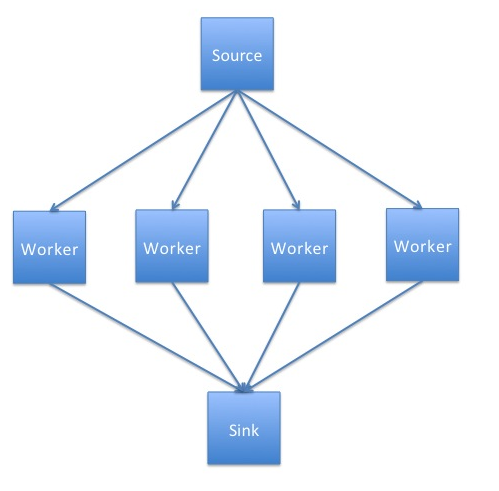
\includegraphics{TFarm.png}}}}
   \caption{Basic Task Farm}
   \label{fig:taskfarm}
\end{figure}


A source process, also known as a master or controller process,  generates a pool of jobs, while a sink process (often combined with the source process) consumes the results of the tasks. A 'farm' of one or more 
workers claim jobs from the source, process the task and dispatch those results to the sink. 

The workers continually claim jobs until the pool is exhausted. When the number of jobs is greater than the number of workers,  load balancing a computation becomes important.



The parts of a task farm:
\begin{itemize}
\item \textbf{Source} creates and distributes tasks.
\item \textbf{Worker} processes tasks and passes on results.
\item \textbf{Sink} gathers results and collates them.
\end{itemize}


\subsection{Using a Task Farm}
Using a task farm is most common in large computations composed of lots of independent calculations and can effectively speed up the overall calculation by using the available processors by assigning tasks to 
them as they request them. This would usually be when a processor finishes a task. 

Allowing that some calculations will take longer than others, it is an effective method for getting more use out of the processors as opposed to using a lock-step calculation method (waiting on the whole set of 
processors to finish a current job) or pre-distributing all tasks at the beginning where all the long tasks could be given to a single processor. 

Using a callback from the worker when it finishes helps to load balance the tasks. Without managing this, all the work could be carried out by a single processor, meaning the overall runtime will be dominated by 
that processor.

\subsection{Not always a Task Farm}
While many problems can be broken down into individual parts, there are a sizeable number of problems where this approach will not work. Problems which involve lots of interprocess communication are ofen not suitable for 
task farms as they require the master to track which worker has which element, and to tell workers which other workers have which elements to allow them to communicate. Additionally, the sink progress may need to track this 
as well in cases of output order dependency. 

It should be noted that task farms are used where there are lots of communications; but the drawbacks and overheads have to be noted in these cases. The examples in this exercise are lots of independent tasks 
which can be collated by the sink process. In this exercise, there are no communications between the worker tasks.

\subsection{Load Balancing} 


Load balancing is how a system determines how work or tasks are distributed across processing elements to ensure good performance. Successful load balancing will avoid overloading a single element, 
maximising the throughput of the system and make best use of resources available. Poor load balancing will lead to elements of the system being under-utilised and reducing the performance as it gets dominated 
by over-subscribed resources.

\subsection{Poor Load Balancing}
\begin{figure}[h] %  figure placement: here, top, bottom, or page
{\centerline{\resizebox{0.70\hsize}{!}{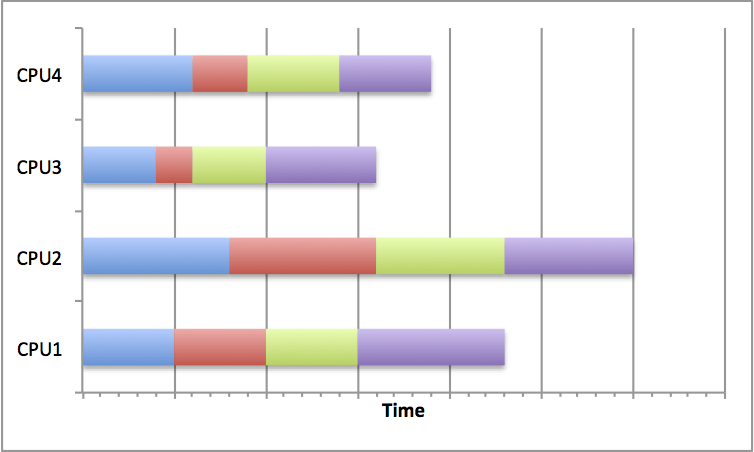
\includegraphics{badbalance.png}}}}
   \caption{Four process task farm with a poor distribution of tasks}
   \label{fig:poorbalance}
\end{figure}

Figure \ref{fig:poorbalance} shows how some distributions of jobs will skew the task completion time. In the diagram it shows that CPU2 has a far longer completion time for its tasks, particularly compared to 
CPU3. This means that the calculation will take longer (as the total runtime is equivalent to the longest runtime on any of the CPUs) and the resources are not being used optimally. This can occur when load balancing is not considered, random scheduling is used (although this is not 
always bad) or poor decisions are made about the job sizes.

\subsection{Good Load Balancing}

\begin{figure}[h] %  figure placement: here, top, bottom, or page
   \centering
{\centerline{\resizebox{0.70\hsize}{!}{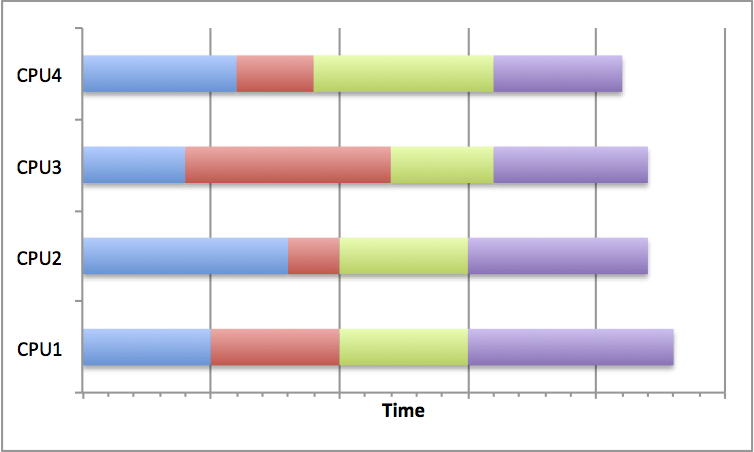
\includegraphics{goodbalance.png}}}}
   \caption{Four process task farm with a good distribution of tasks}
   \label{fig:goodbalance}
\end{figure}

Figure \ref{fig:goodbalance} shows how by scheduling jobs carefully, the best use of the resources can be made. By choosing a distribution strategy to optimise the use of resources, the CPUs in 
the diagram all complete their tasks at roughly the same time. This means that no one task has been oversubscribed and dominated the running time of the overall calculation. This can be achieved by many 
different means. 

Where the task sizes and running time are known in advance, the jobs can be scheduled to allow best resource usage. The most common distribution is to distribute large jobs first and then distribute 
progressively smaller jobs to equal out the workload. 

If the job sizes can change or running time is unknown, then an adaptive system could be used which tries to infer future task lengths based upon observed runtimes.

The program in this exercise uses an approach where a set of tasks form a queue and as each worker finishes a task it takes the next one from the top of the queue. This load balances by ensuring that a worker with short tasks will take more to complete compared to a worker with long tasks.

\subsection{Quantifying the Load Imbalance}

We can try an quatify how well balanced a task farm is by computing
the {\em Load Imbalance Factor}. We look at the loads of the different workers and compute:
\[
Load\ Imbalance\ Factor = \frac{workload\ of\ most\ loaded\ worker}{average\ workload\ of\ workers}
\]

For a perfectly load-balanced calculation this will be equal to 1.0;
in general, it will be greater than 1.0.

It is a useful measure because it allows you to predict what the
runtime would be for a perfectly blanced load on the same number of
workers, assuming that balancing the load incurs no additional
overeheads.

For example, if the load imbalance factor is 2.0 then this implies
that the runtime can in principle be halved by better load balancing.

\newpage

\section{Exercise}

There are three main tasks to accomplish in this exercise: Compilation,
Initial Run and Run Tests.

\subsection{Compilation}

First, log on to the ARCHER frontend as before. Use \verb+wget+ to
obtain the file \verb+fractal.tar.gz+ from the ARCHER course material
pages. Make sure that you are in your \verb+/work/+ filesystem on
ARCHER.

To compile the code, switch to the {\verb+fractal+}
directory and issue the make command.

\begin{lstlisting}[frame=single]
  guestXX@archer:~> make
  cc -g -c arralloc.c
  cc -g -c fractal.c
  cc -g -c read_options.c
  cc -g -c write_ppm.c
  cc -g -o fractal arralloc.o fractal.o read_options.o write_ppm.o -lm
\end{lstlisting}

After compilation a executable file will have been created called \textbf{fractal}.

\subsection{Initial Run}

\textbf{Remember} you will need to submit a job using a batch
script. A working batch script is provided for you, but you will need
to modify it to change, for example, the number of workers or the
number of tasks. This involves changing \verb+aprun+ command as
  detailed below.

\subsubsection{Starting Off}
The fractal executable will take a number of parameters and
produce a fractal image in a file called \verb+output.ppm+. The image will be
banded in different shades which show which processor did which
section. This allows how the tasks were allocated to be observed. An
example of this is presented in figure \ref{fig:example}.

The executable can take a number of parameters which will determine
how the program functions, but we are mainly interested in the varying
the number of tasks so we will use the default values for the other
parameters (see Section~\ref{sec:fracparams} for a complete list of the
options).

The default submission script does the following:
\begin{lstlisting}
  aprun -n 17 ./fractal -t 192
\end{lstlisting}

This creates a task farm with one master process and 16 workers. It
divides the image up into tasks, where each task is a square of the size of 
192 by 192 pixels. The default image size is $768 \times 768$ pixels,
so this means there is exactly one task per worker, i.e. we are not
yet doing anything to balance the load.

\begin{figure}[h] %  figure placement: here, top, bottom, or page
{\centerline{\resizebox{0.70\hsize}{!}{
\includegraphics{example1.png}}}}
   \caption{Example image with more tasks (256) than workers (16)}
   \label{fig:example}
\end{figure}

Submit your job to the batch system using the commnad:
\begin{lstlisting}
  guestXX@archer:~> qsub -q course1 fractal.pbs
  58306.sdb
\end{lstlisting}

\textbf{Remember} the number returned *****.sdb is the job ID. 

\textbf{Remember} you can monitor the progress of your job in the batch queue using 
\begin{verbatim}
qstat -u $USER
\end{verbatim}

Once the program has successfully completed the directory you are working in should contain the file fractal.o<jobID> with the following output:



\begin{lstlisting}[frame=single]
Number of processes:                     17
Image size:                      768 x 768 
Task size:                       192 x 192 (pixels)
Number of iterations:            5000
Coordinates in X dimension:      -2.000000 to 1.000000
Coordinates in Y dimension:      -1.500000 to 1.500000

-----Workload Summary (number of iterations)---------

Total Number of Workers: 16
Total Number of Tasks:   16

Total   Worker Load: 498023053
Average Worker Load: 31126440
Maximum Worker Load: 156694685
Minimum Worker Load: 62822

Time taken by 16 workers was 1.926423 (secs)
Load Imbalance Factor: 5.034134

\end{lstlisting}


The loads of the workers are estimated as the total number of
iterations of the Mandelbrot calculation summed over all the pixels
considered by that worker. The assumption is that the time taken is
proportional to this.
The only time that is actually measured is the total time taken to
complete the calculation.


You can view the output file using
 \verb+display output.ppm+, an example of which is found in figure \ref{fig:example}.

\subsection{Run Tests}

In the Using HPC Resources exercise, there were a series of questions
to explore about how speedup is considered, how well the code actually
scales and how cheaply something could be run quickly. This involved
doing multiple runs to get better average runtimes. In this case these
questions are important, but workload and load balance is very
important here. It is best to get maximum use out of resources and not
pay for resources which are not doing work. So there are a series of
questions to explore here:

\begin{enumerate}
\item From the default run with 16 workers and 16 tasks, what is your predicted best run time based on the Load Imbalance Factor?
\item Increase the number of tasks by decreasing the task size and note the runtimes
\item Does the runtime approach what you predicted?
\item Look at the output for 16 tasks: can you understand how the load was distributed across workers by looking at the colours of the bands and the structure of the Mandelbrot set?
\item Are the results qualitatively different if you use more workers?
\item Experiment with varying the parameters, e.g. using the Julia set rather than the Mandelbrot set.
\end{enumerate}

If you are only interested in looking at the output picture it is best
to use the \textbf{-n} option to the \textbf{fractal} program - see
Section~\ref{sec:fracparams}.

\textbf{Remember} that the black areas {\em inside} the Mandelbrot set are {\em
  expensive} to compute. The red areas {\em outside} the set are {\em cheap} to compute.

\section{\label{sec:fracparams}Fractal Parameters}

The number of workers is set by the \textbf{-n} argument to
\textbf{aprun}; the number of workers is one fewer than the number of
processes as we require one process to be the controller.

The following options are recognised by the \textbf{fractal} program
itself:

\begin{itemize}
\item \textbf{-S} number of pixels in x-axis of image.
\item \textbf{-i} maximum number of iterations.
\item \textbf{-x} the x-minimum coordinate.
\item \textbf{-y} the y-minimum coordinate.
\item \textbf{-X} the x-maximum coordinate.
\item \textbf{-Y} the y-maximum coordinate.
\item \textbf{-f <fractal function>} (set to J for Julia set)
\item \textbf{-c} the real part of the parameter $c + i C$ for the Julia set.
\item \textbf{-C} the imaginary part of the parameter $c + i C$ for the Julia set.
\item \textbf{-t} task size (pixels $\times$ pixels).
\item \textbf{-n} do not shade the output image based on task allocation to workers.
\end{itemize}

The Wikipedia page on the Julia Set has some suggestions for interesting parameters.
For example, try:
\begin{verbatim}
aprun -n 17 ./fractal -t 96 -n -f J -c -0.8 -C 0.156 -x -2 -X 2
\end{verbatim}

\nocite{*}
\bibliography{reff}{}
\bibliographystyle{plain}

\end{document}

